\chapter{Appendix B - Hardware and Firmware}


\section{Schematics}

LearnAir V2 schematics are below.

\FloatBarrier

\begin{figure}[htb]
 	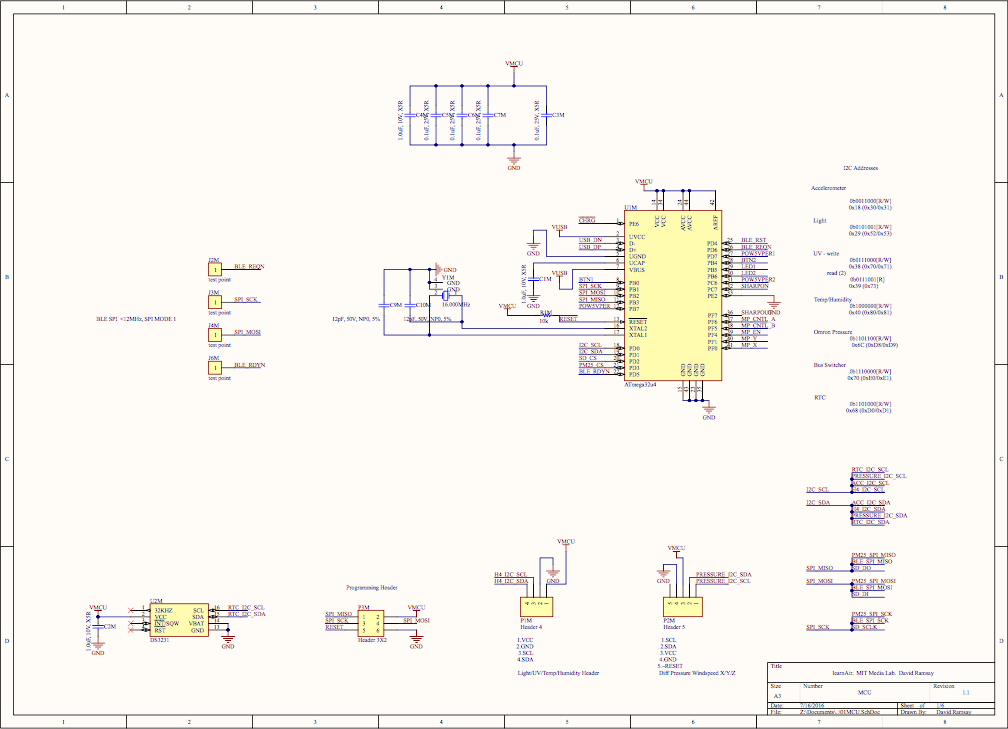
\includegraphics[width=\textwidth + \marginparwidth]{schematics/la_schematic1}               
\end{figure}
\begin{figure}[htb]
 	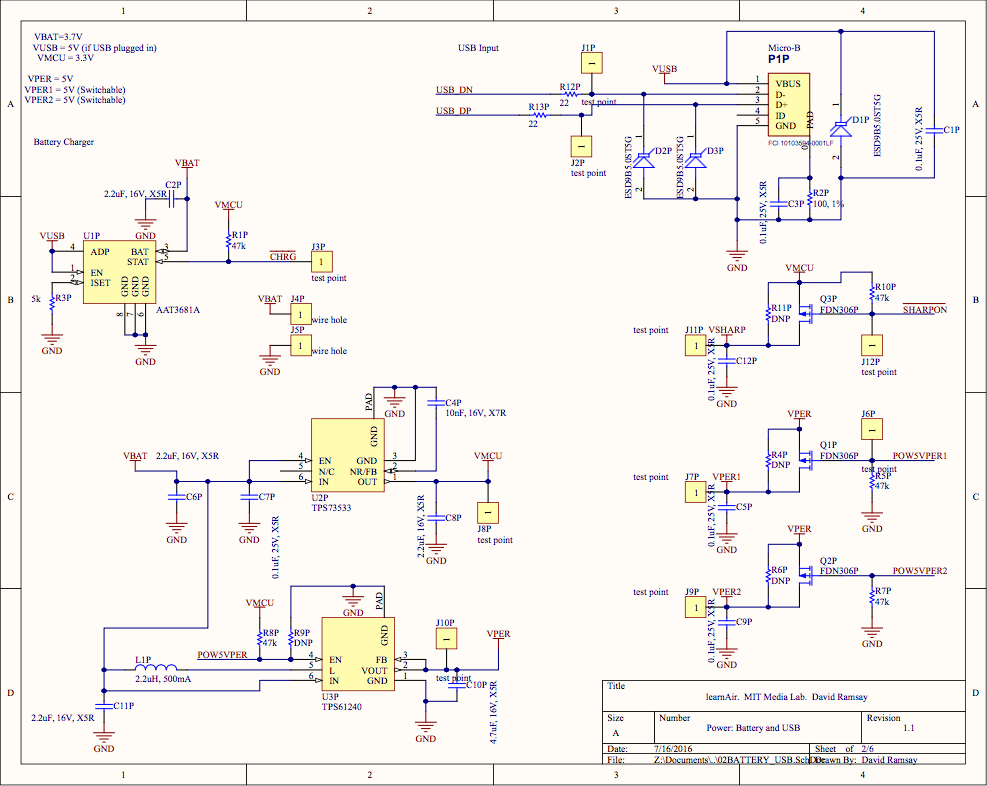
\includegraphics[width=\textwidth + \marginparwidth]{schematics/la_schematic2} 
 	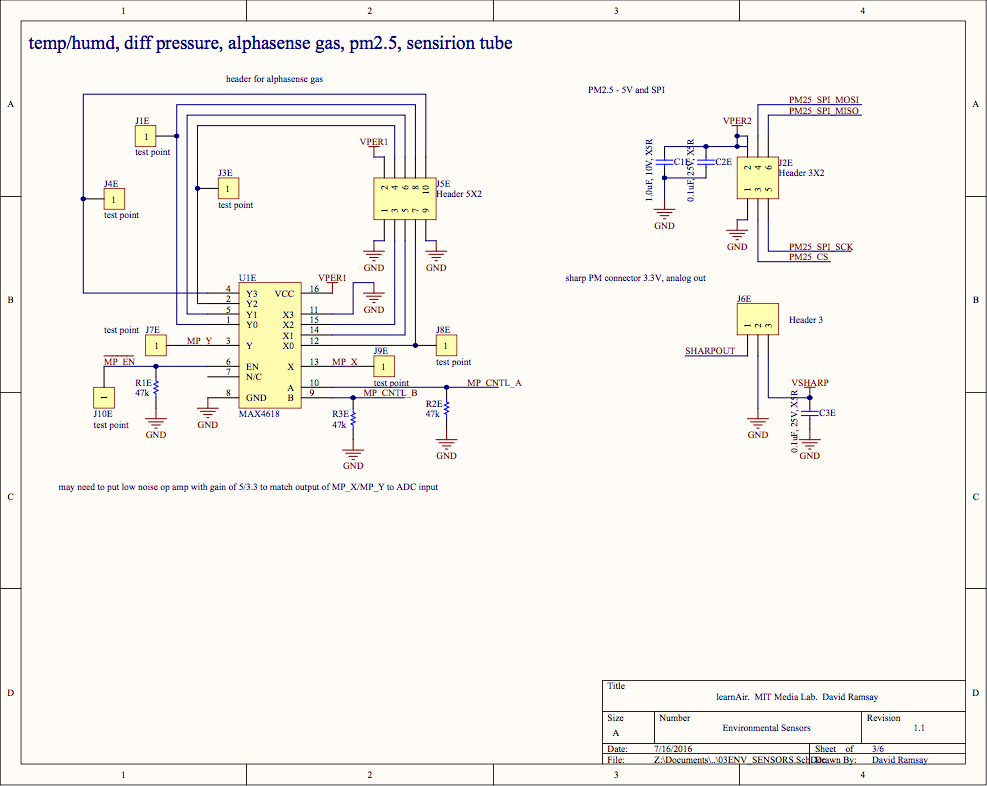
\includegraphics[width=\textwidth + \marginparwidth]{schematics/la_schematic3}                 
\end{figure}

\begin{figure}[htb]
 	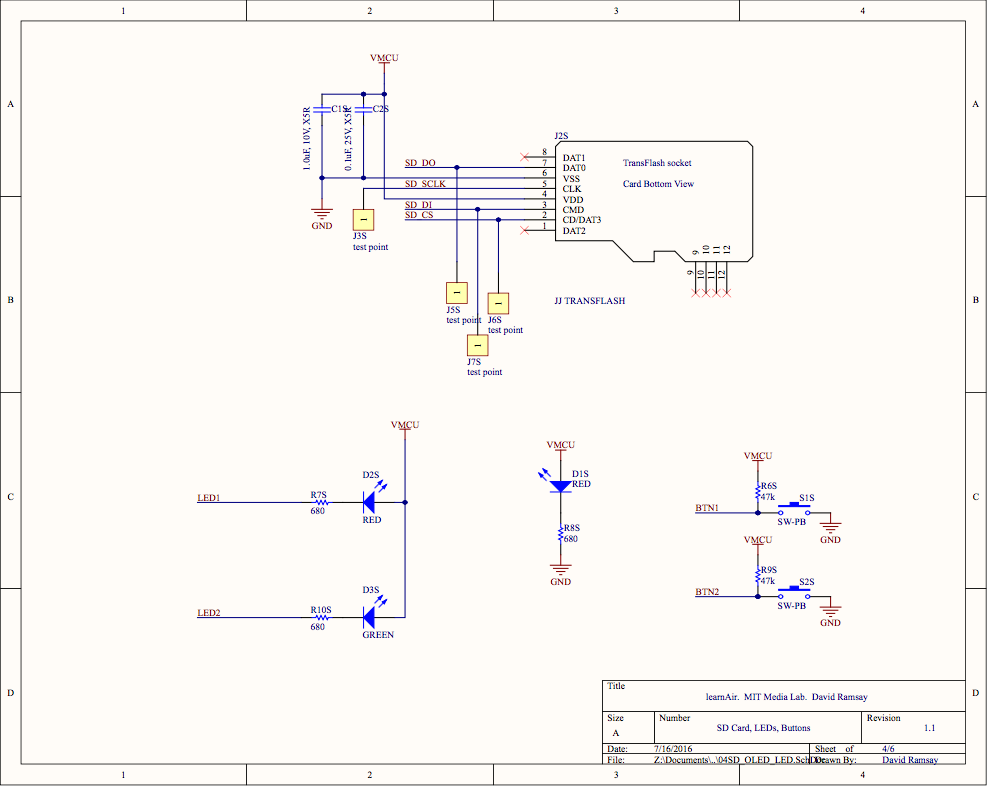
\includegraphics[width=\textwidth + \marginparwidth]{schematics/la_schematic4} 
 	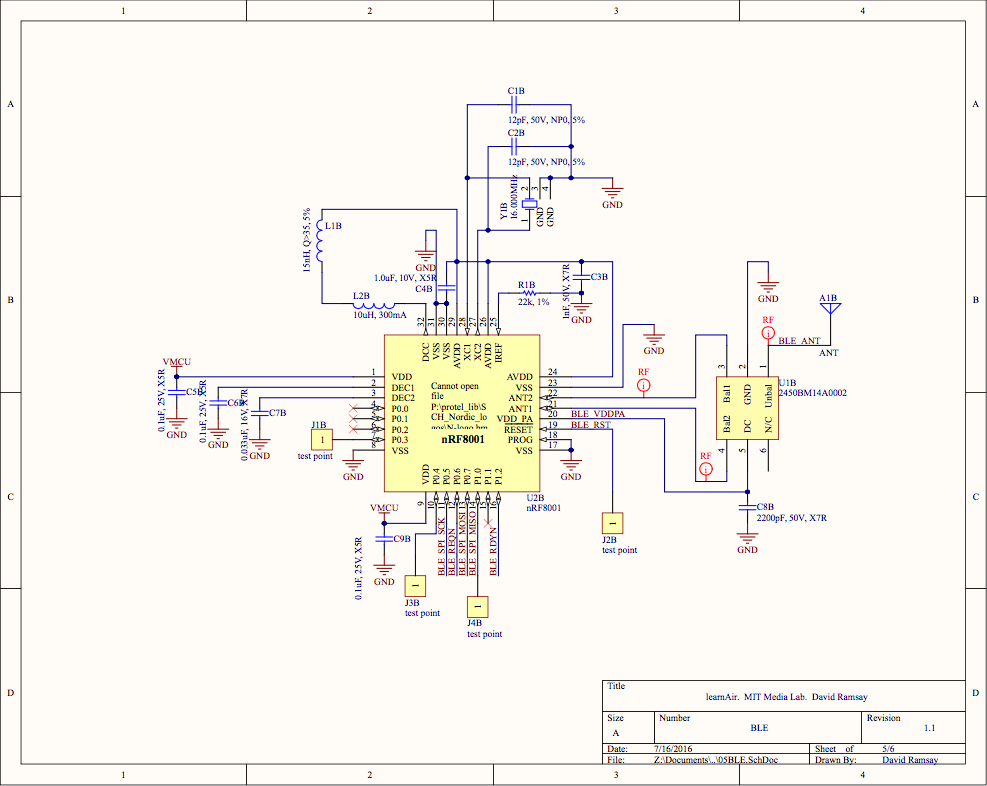
\includegraphics[width=\textwidth + \marginparwidth]{schematics/la_schematic5}              
\end{figure}
\begin{figure}[htb]
 	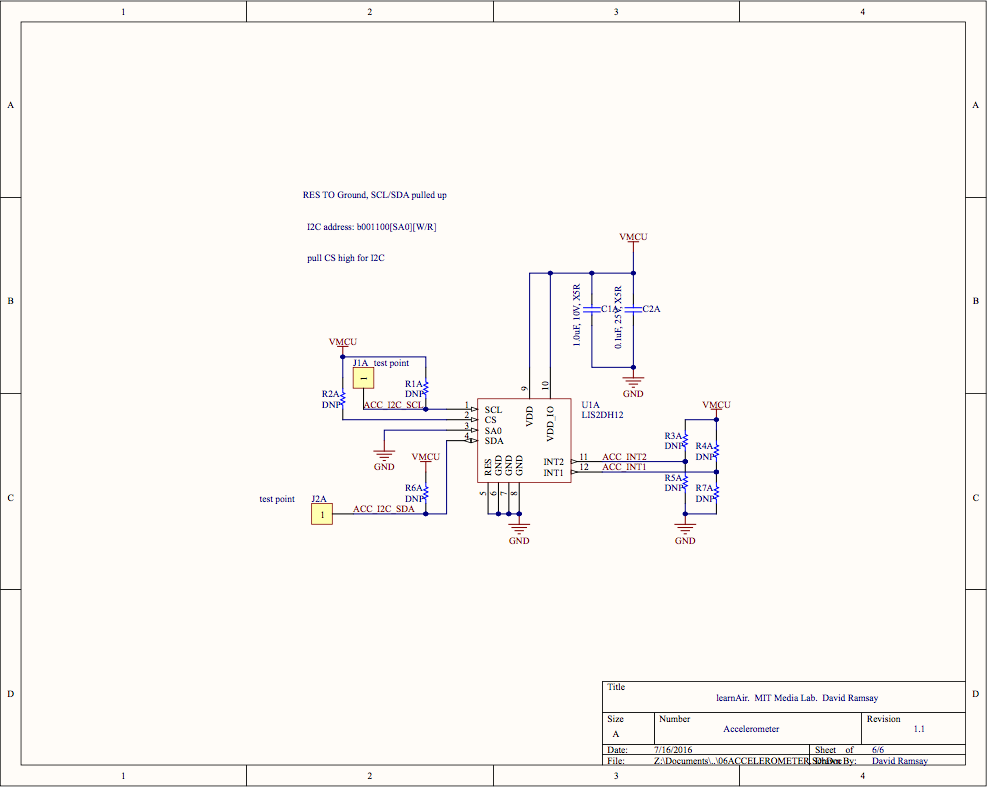
\includegraphics[width=\textwidth + \marginparwidth]{schematics/la_schematic6}               
\end{figure}

\FloatBarrier
LearnAir V3 uses the same schematics for peripherals, power, accelerometer, and BLE as for LearnAir V2.  The two differing schematics (MCU and SD Card) are shown below. 
\FloatBarrier

\begin{figure}[htb]
 	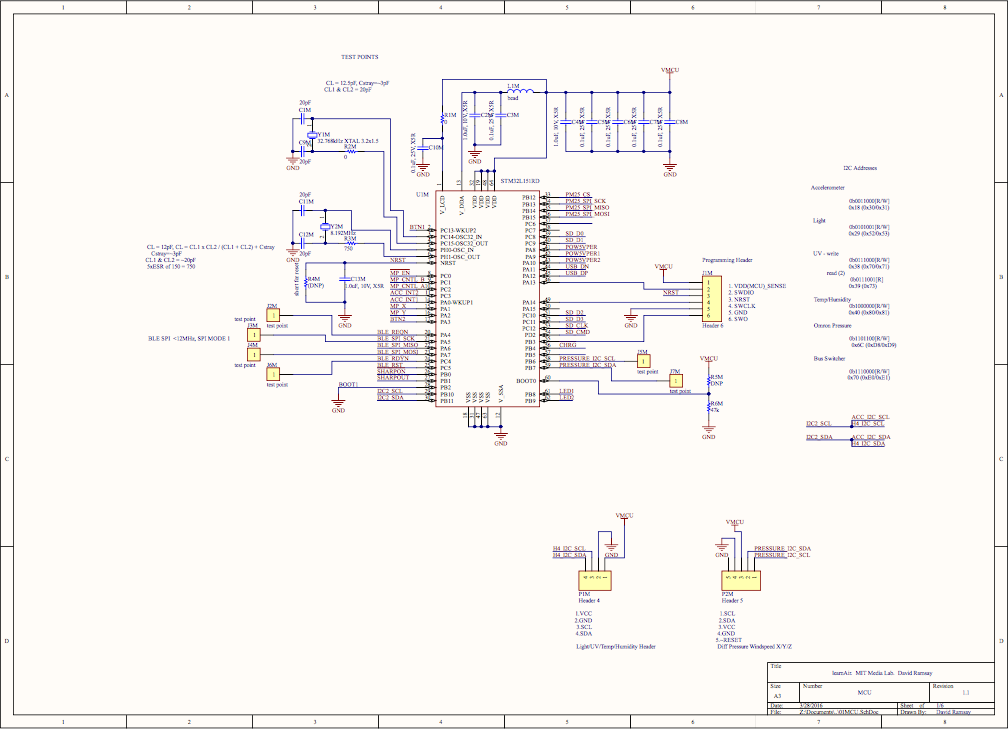
\includegraphics[width=\textwidth + \marginparwidth]{schematics/l3_schematic1}            
\end{figure}

\begin{figure}[htb]
	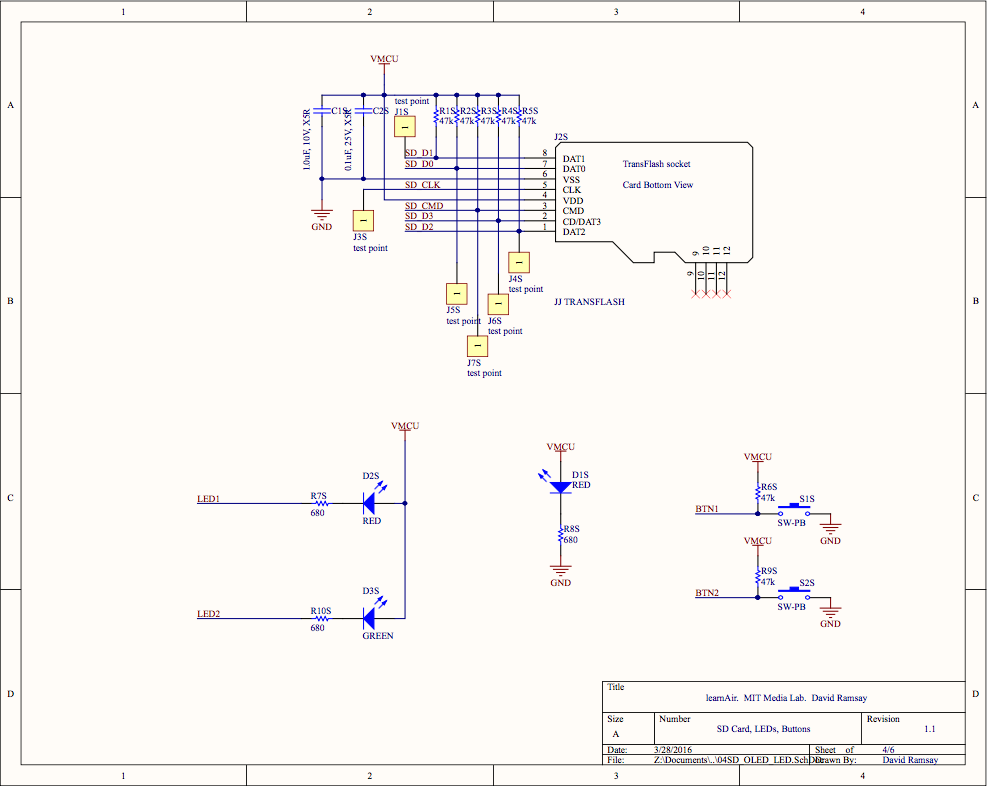
\includegraphics[width=\textwidth + \marginparwidth]{schematics/l3_schematic2}     
\end{figure}

\FloatBarrier
\section{Firmware}
\FloatBarrier

\FloatBarrier
\section{Hardware Analysis}
\FloatBarrier

Figure \ref{fig:ws_with_10_accuracy} shows the windspeed measurement comparison between our conditioned pressure sensor measurement and the MassDEP windspeed measurement. Within $\pm$5\% is denoted with green highlights.

\begin{figure}[htb]
 	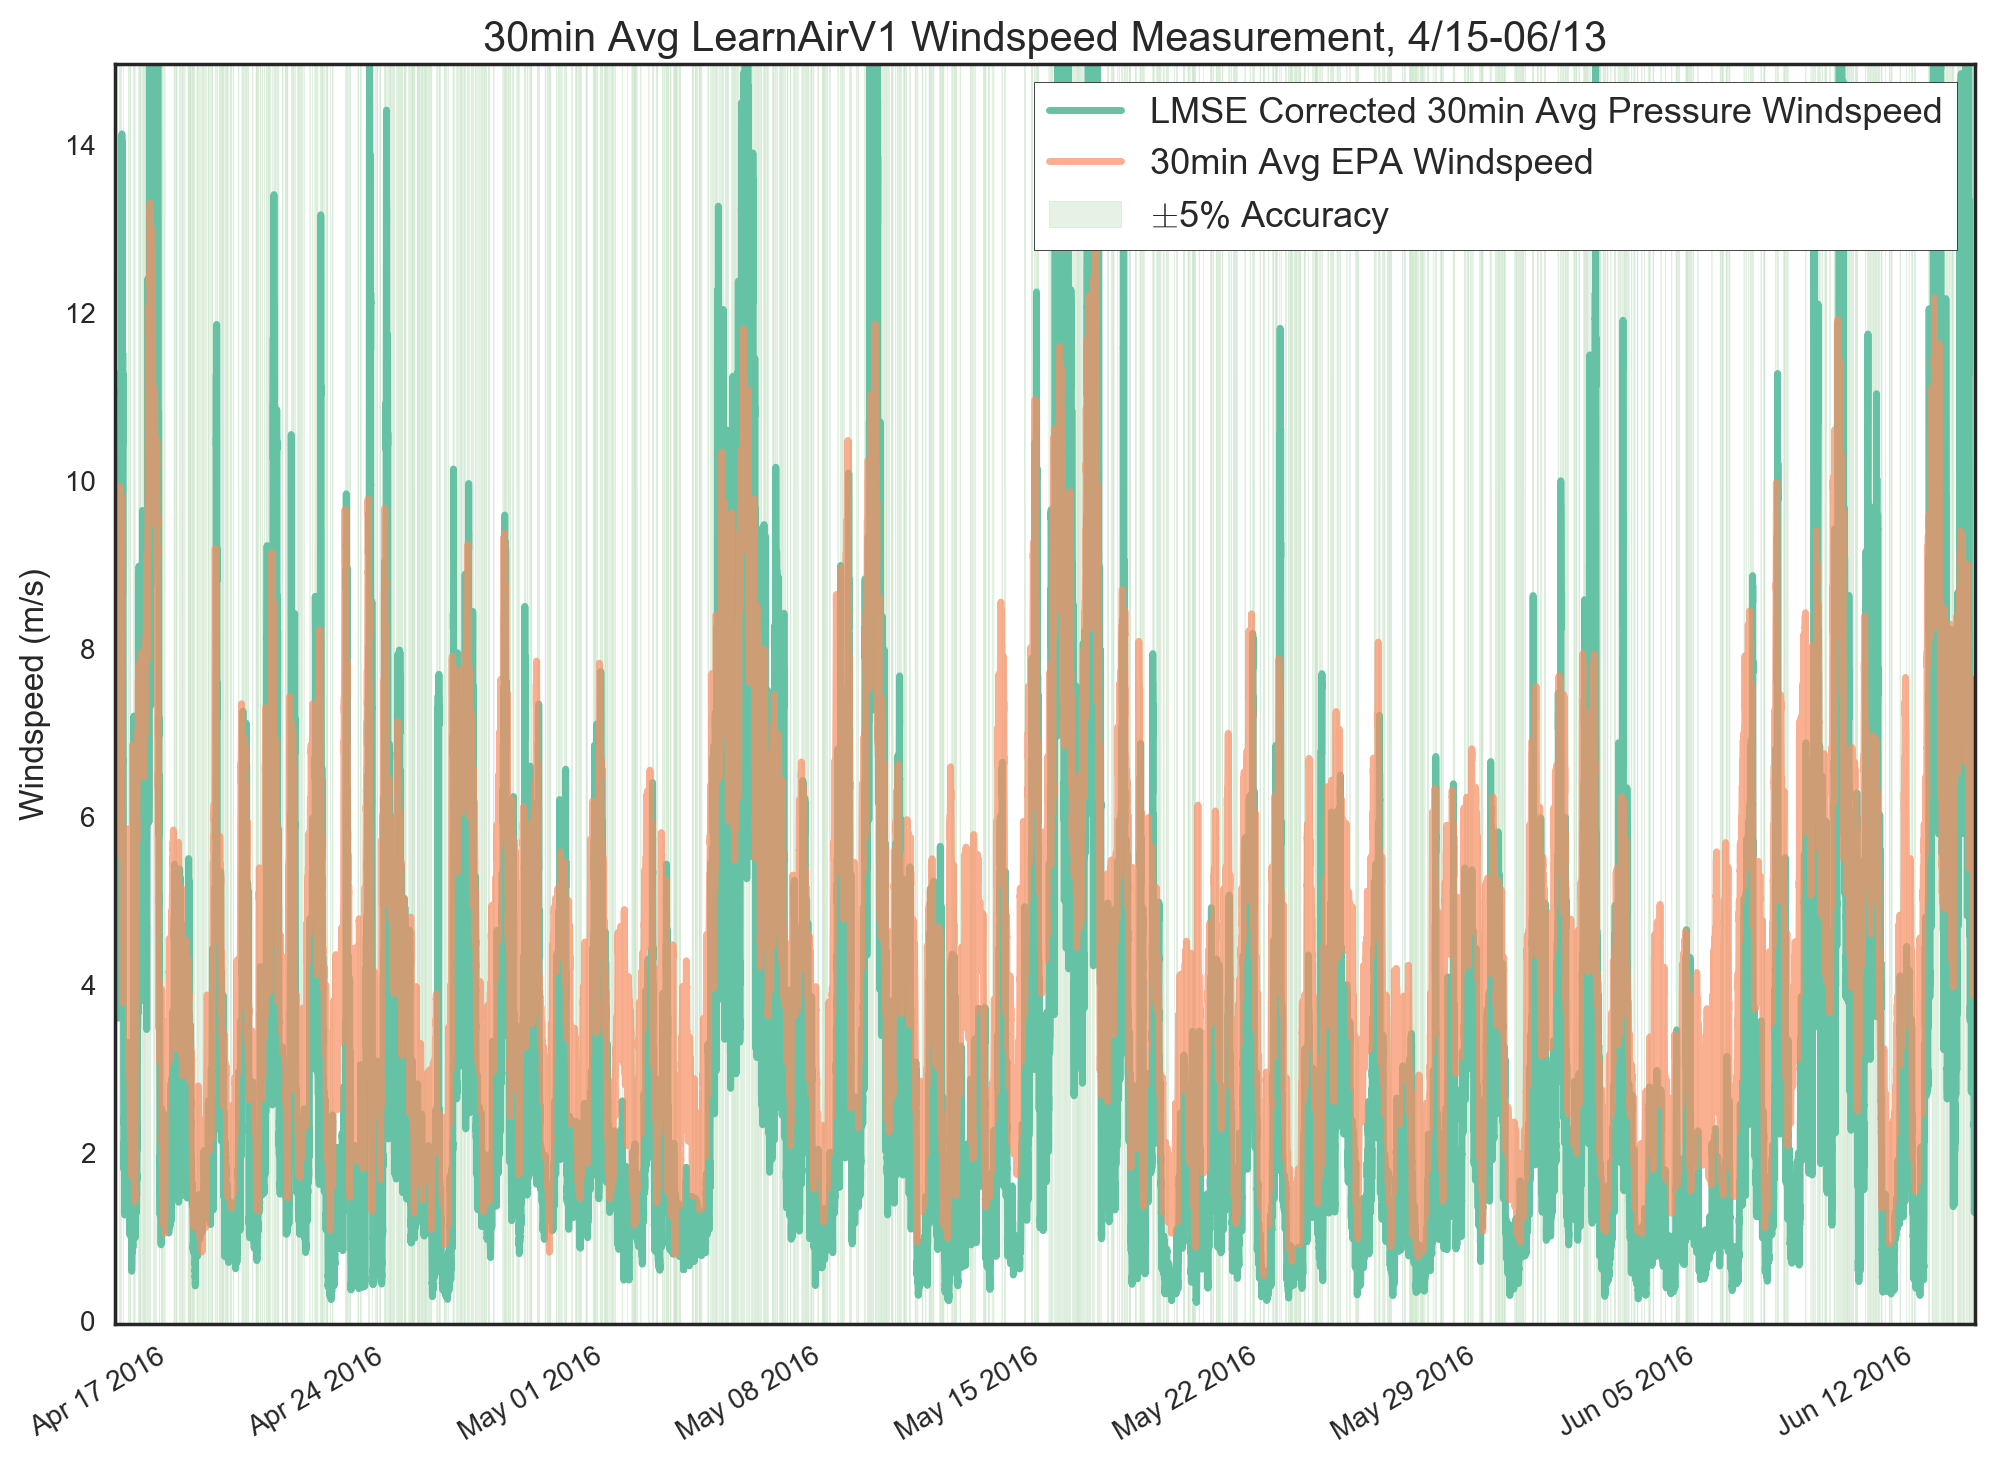
\includegraphics[width=\textwidth]{figs/ws_with_10_accuracy}               
 	 \caption{Wind Speed Measurement with 10\% Accuracy}
  	\label{fig:ws_with_10_accuracy}
\end{figure}

Figure {\ref{fig:wd_with_10_accuracy_zoomed} shows the wind direction angle over the course of a day, with an indication of how closely the conditioned wind pressure sensor reading matched the actual windspeed.  Green highlighting indicates that our windspeed measurement was within $\pm$5\% of the MassDEP reading.  This plot is useful to look for systemic errors-- are there any wind directions where we consistently are accurate in our measurment?  Are there any wind directions where we're inaccurate?  It appears there are no obvious relationships between wind direction and accuracy from this graph.  However, there are interesting relationships between wind direction and error-- please see Chapter 5.
 
\begin{figure}[htb]
 	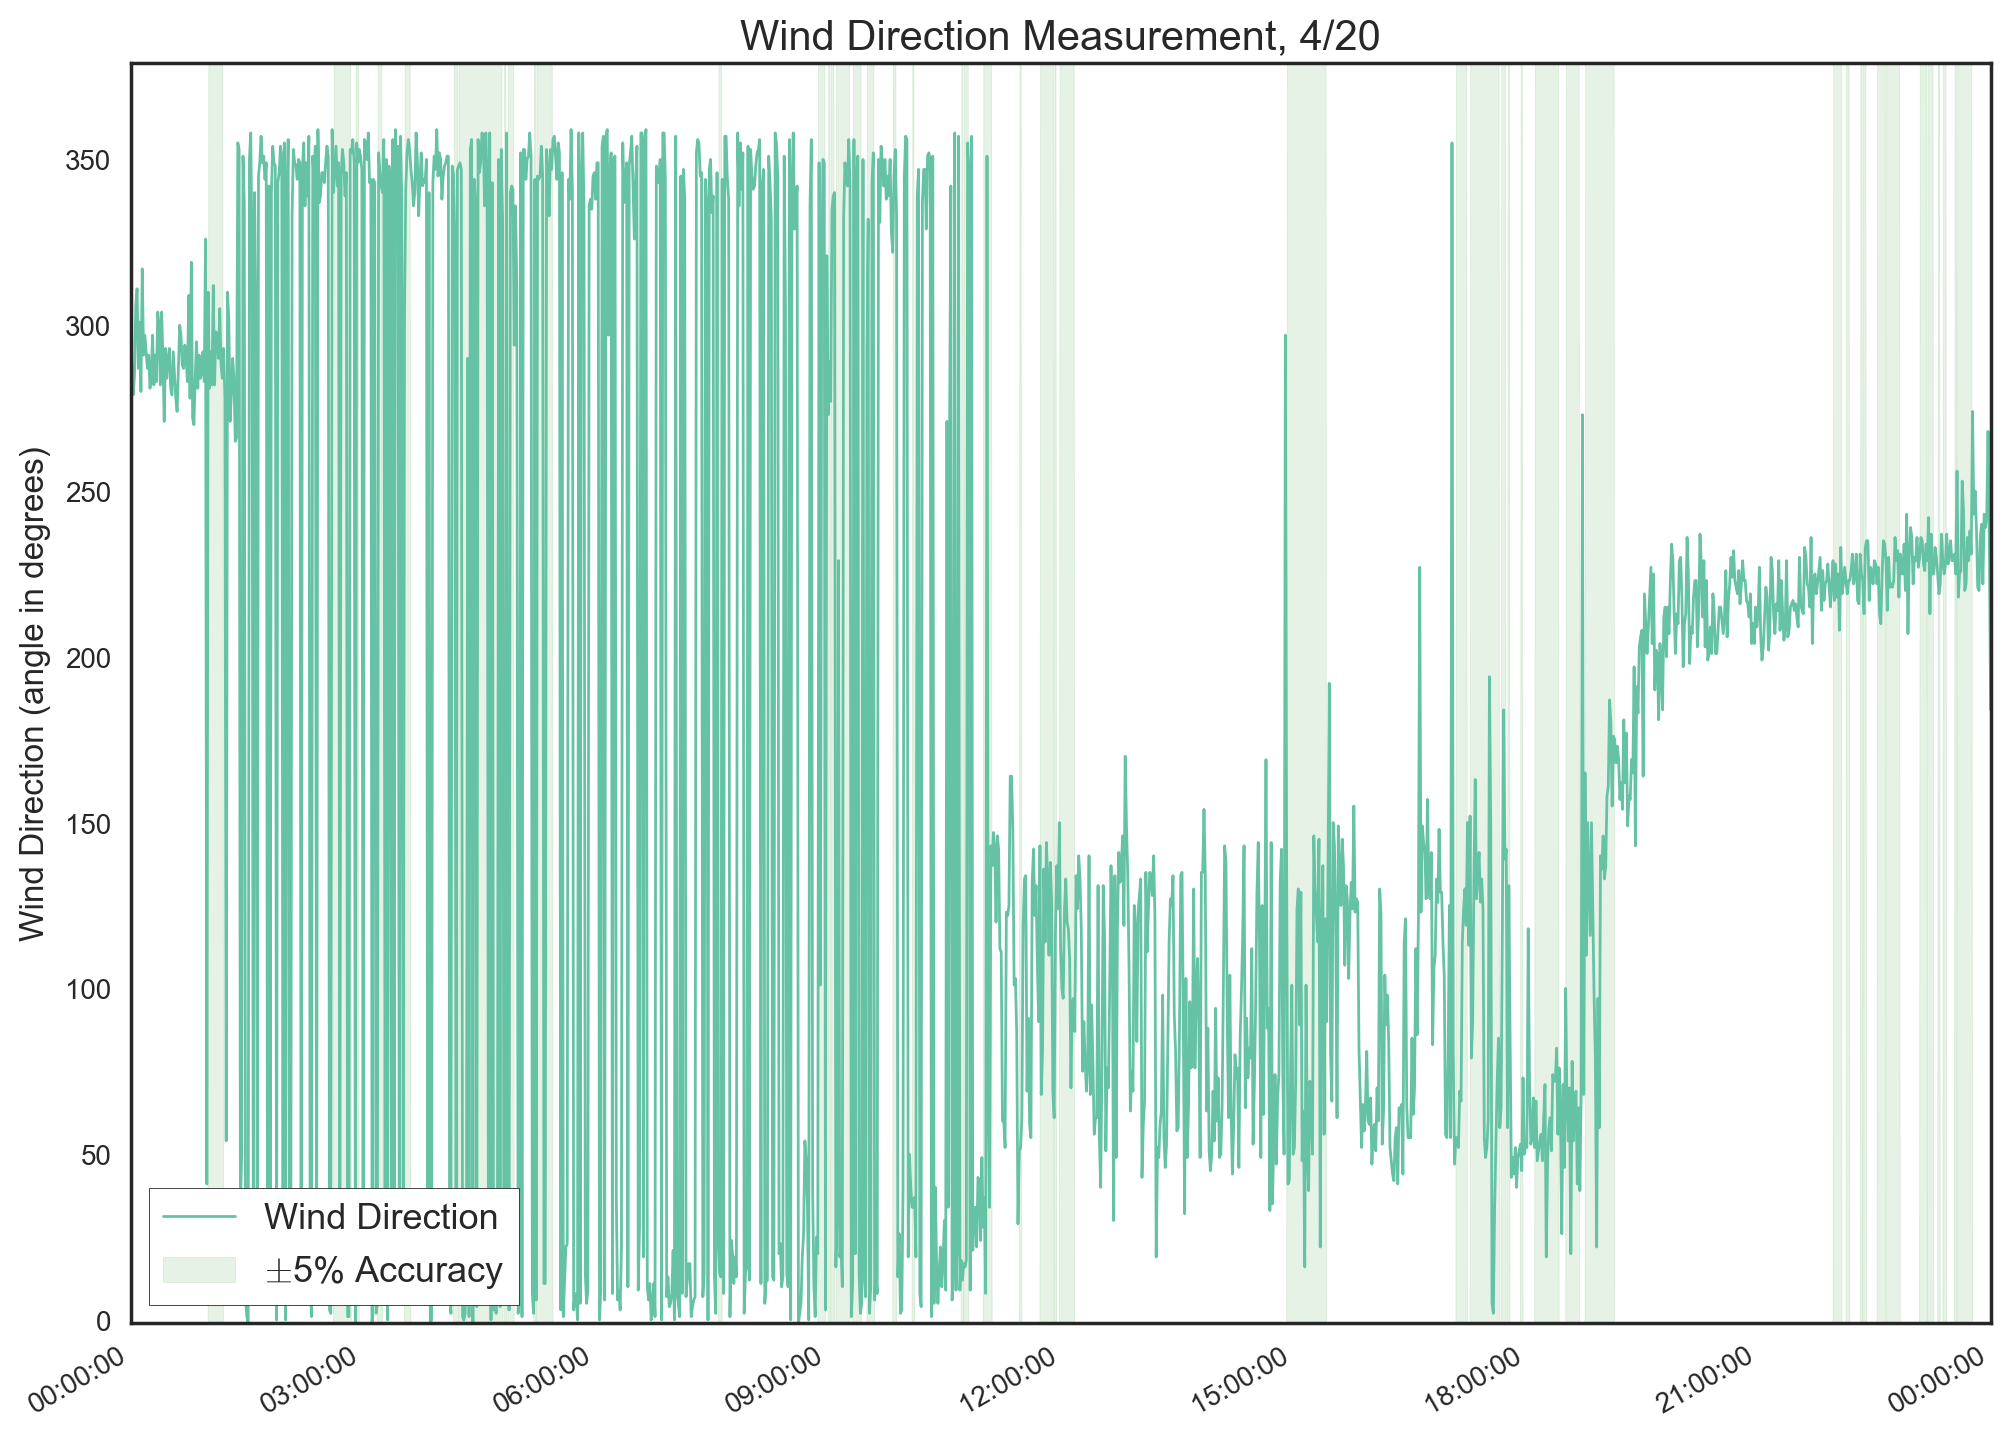
\includegraphics[width=\textwidth]{figs/wd_with_10_accuracy_zoomed}               
 	 \caption{Wind Direction with 10\% Accuracy WindSpeed Measurements Denoted}
  	\label{fig:wd_with_10_accuracy_zoomed}
\end{figure}

\clearpage
\newpage
